\subsection{Camera Input}
\label{sec:camera_discussion}
In the early stages of the project,
we looked at various camera modules on-line and tried to assess how they would work in our system.
Some modules were very simple, and some had many features.
The PiCamera was the most feature-complete module we looked at.
When we looked into the camera control protocol for the PiCamera,
we found \textit{some} information about it,
like the open source C and Python camera control libraries for the Raspberry Pi
and the pin-outs for the ribbon connector.
From what found, it was assumed that it would be possible to implement camera control with the MCU or FPGA.

When the time came to make a choice for the camera module and order it,
the PiCamera was the only option that was available from the retailers we were using,
so the choice was easy.

Had we looked for more information about the PiCamera on-line before this,
we would have perhaps found the Raspberry Pi engineer recommending not using the PiCamera for an FPGA project\footnote{\url{https://www.raspberrypi.org/forums/viewtopic.php?t=119977&p=812191}} or the unclaimed \$1000 bounty for an open-source driver for the PiCamera\footnote{\url{https://parallella.org/forums/viewtopic.php?f=10&t=2514}}.
This would have indicated that we should have looked for another camera module.

\subsubsection{MCU as Camera Controller}
% \begin{figure}
%     \centering
%     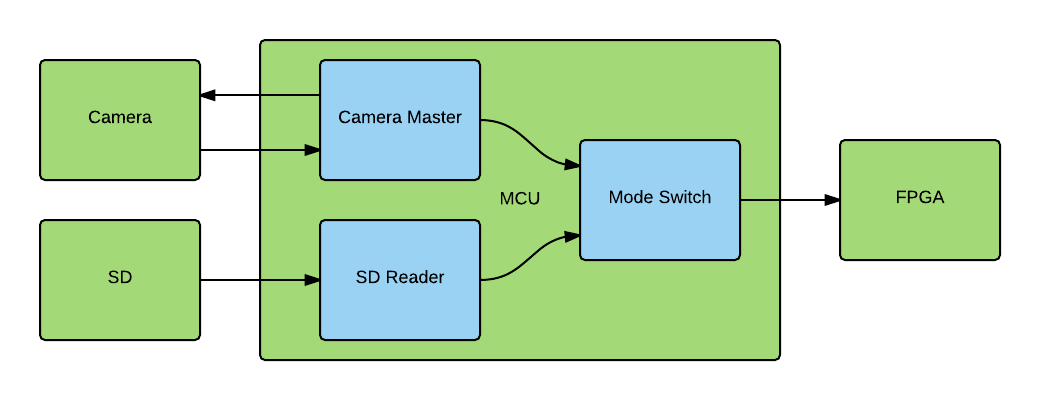
\includegraphics[width=\linewidth]{img/MCU_CameraMaster}
%     \caption{MCU as input controller. Hardware components in green, software components in blue.}
%     \label{fig:MCU_CameraMaster}
% \end{figure}

The first option explored was to have the MCU be the camera controller and receive the video stream.
This idea was abandoned eventually as the EFM32GG does not have hardware to receive the differential bus data,
so the FPGA would be more appropriate for this role.

\subsubsection{FPGA as Camera Controller}
% \begin{figure}
%     \centering
%     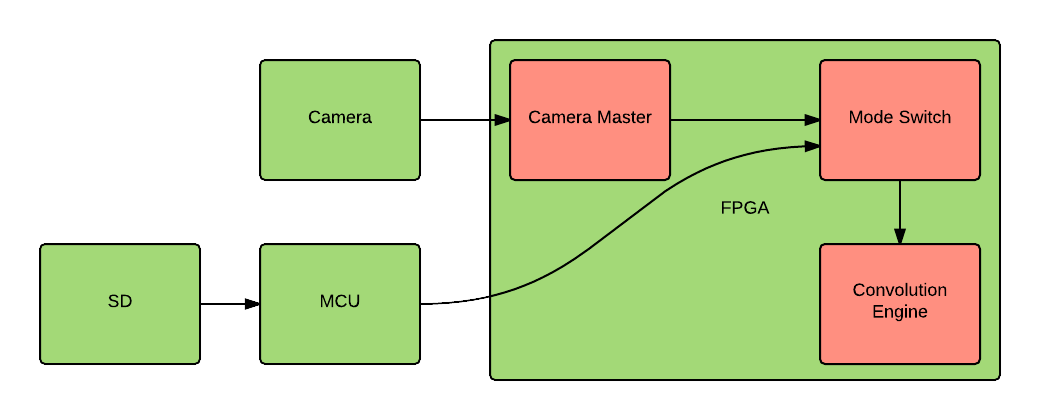
\includegraphics[width=\linewidth]{img/FPGA_CameraMaster}
%     \caption{FPGA with input controller module. Hardware components in green, FPGA sub-modules in red.}
%     \label{fig:FPGA_CameraMaster}
% \end{figure}

After aquiring a snapshot of the I2C communication between the Pi and the PiCamera with a logic analyser,
a VHDL module was written that could output the same sequence,
and this was tested with the Spartan-6 development board and the PiCamera.
While the FPGA was able to output the I2C sequence,
the camera would not send acknowledgements for any of the transmissions.
Efforts into figuring out why the PiCamera wouldn't respond were fruitless, so the idea was eventually abandoned.

\paragraph{Using the Raspberry Pi}
Since reverse-engineering the camera control protocol was difficult,
we tried to use a Raspberry Pi to control the camera,
then transfer the video stream to the Camvolution board.
The provided software on the Pi makes it very easy to have full control of the camera,
but transferring video out of the Pi at high rates is more challenging.

\paragraph{GPIO Pins}
The Raspberry Pi has GPIO pins that are controllable in software.
A script was written which could output pixel data to the GPIO pins as a parallel bus with one clock pin and eight data pins.
This was very simple to implement, however it was also very slow.
With a Raspberry Pi 2 the best clock frequency achieved on this bus was approximately $600kHz$.
This would only allow sending very small frames of video at low frame rates.

The Raspberry Pi also has hardware support for SPI over some of the GPIO pins.
Directing the video stream to this instead was more promising,
since the frequency of the clock in this mode would be able to go up to $32MHz$\footnote{\url{http://elinux.org/index.php?title=RPi\_SPI\#Speed\_2}},
which would be a massive improvement even if the transfer was serial instead of 8-bit parallel.
Unfortunately what was observed was that while the transfer of chunks of data was fast,
there were long delays between chunks.
At 240x240 resolution, 6 frames per second was the best transfer rate that was able to keep up with the recording.
Figures \ref{fig:Logic7fps} and \ref{fig:Logic1Frame} shows the logic analyser output for SPI transfers.

\begin{figure}
    \centering
    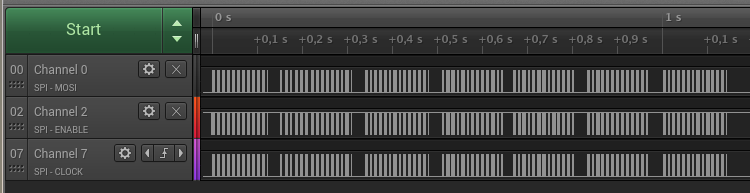
\includegraphics[width=\linewidth]{img/logic/7fps}
    \caption[7 FPS SPI transmission]{
        At 7 FPS recorded, the SPI transmission is unable to keep up and sends the seventh frame too late.
    }
    \label{fig:Logic7fps}
\end{figure}

\begin{figure}
    \centering
    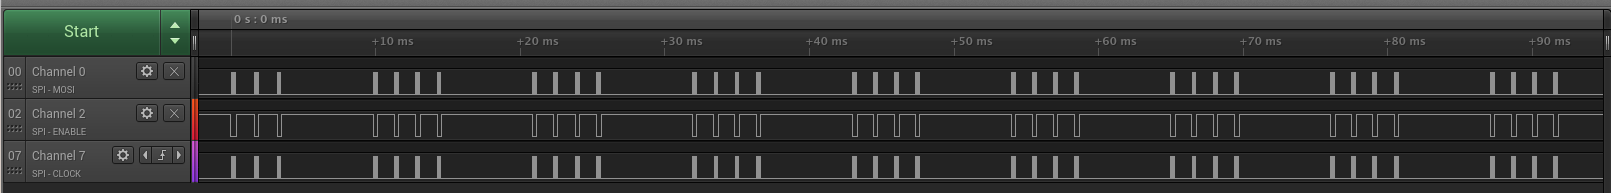
\includegraphics[width=\linewidth]{img/logic/1frame}
    \caption[Idle time between SPI transmissions]{
        Inspecting a single frame transmission closer reveals a lot of idle time.
    }
    \label{fig:Logic1Frame}
\end{figure}

\paragraph{HDMI Output}
Seeing that all efforts into using the camera were either failing or at best offering a tiny stream of data,
we decided to concentrate on the HDMI input of the Camvolution system.
The Raspberry Pi has HDMI out, so it would definitely be possible to use the PiCamera with this set-up.
